\documentclass{Class/julia}

\usepackage{geometry}
\usepackage{graphicx} % To use \resizebox
\usepackage{array} % For custom column widths
\usepackage{calc} % To use \widthof

\usepackage{siunitx} % Formatting numbers in a table

\usepackage{amsmath}
\usepackage{subcaption}
\usepackage{threeparttable}
\usepackage{hyperref}
\usepackage{listings}
\usepackage{xcolor}
\usepackage{multirow}
%\usepackage{placeins}

\geometry{
    a4paper,
    total={170mm,257mm},
    left=20mm,
    top=20mm,
}

\author{Julia Maria Wdowinska}
\date{} % Remove date from the title

\begin{document}

\begin{titlepage}
    \centering
    \vfill
    {\scshape\Large University of Milan \par}
    \vspace{0.5cm}
    {\scshape\large Faculty of Political, Economic and Social Sciences \par}
    \vspace{3cm}
    {\huge
    \textbf{Parallelized SON Algorithm for Frequent Itemset Mining on Large Datasets} \\
    \vspace{0.5cm}
    \large Final Project in the Module Algorithms for Massive Data \par}
    \vspace{2cm}
    {\large \textbf{Julia Maria Wdowinska} \par}
    \vspace{0.5cm}
    {\large Data Science for Economics \par}
    {\large II year\par}
    {\large Master’s Degree \par}
    {\large Matriculation Number:\ 43288A \par}
\vfill
\begin{center}
\begin{figure}[h!]\centering
 
\includegraphics[keepaspectratio=true,scale=0.2]{logo} \\
\end{figure}
\end{center}
\vfill
\begin{center}
{\small{I declare that this material, which I now submit for assessment, is entirely my own work and has not been taken from the work of others, save and to the extent that such work has been cited and acknowledged within the text of my work, and including any code produced using generative AI systems. I understand that plagiarism, collusion, and copying are grave and serious offences in the university and accept the penalties that would be imposed should I engage in plagiarism, collusion or copying. This assignment, or any part of it, has not been previously submitted by me or any other person for assessment on this or any other course of study.}}
\end{center}
\vfill
    {\large \today \par}
    \vfill
\end{titlepage}

\tableofcontents
%\newpage

\section{Introduction}

Frequent itemset mining is an interesting task in data mining. The goal is to identify sets of items that frequently appear together in a dataset, enabling valuable insights such as co-purchase behavior in retail or user preferences in recommendation engines.

Various frequent itemset mining algorithms exist, each with its own advantages. This report presents an implementation of the SON algorithm \citep{savasere1995efficient}, where the Apriori algorithm \citep{agrawal1994fast} is used for local itemset mining, and the solution is parallelized using Apache Spark. The methodology is applied to a dataset of Amazon book reviews \citep{amazon_books_reviews} to identify books that are frequently \textit{liked} together by users. Additionally, the implementation is tested for efficiency across varying dataset sizes, minimum support thresholds, and maximum itemset sizes.

The report is structured as follows:\ Section \ref{sec:2} provides an overview of the algorithms and their implementa- tion. Section \ref{sec:3} introduces the dataset and preprocessing steps. Section \ref{sec:4} presents experimental results, including frequent itemset mining outcomes and scalability tests. Finally, Section \ref{sec:5} summarizes key findings and discusses potential future improvements.

\section{Frequent Itemset Mining Algorithms}\label{sec:2}

\subsection{Apriori Algorithm}

The Apriori algorithm is a classical approach to frequent itemset mining. It takes as input a dataset of baskets - each represented as a set of items - and a minimum support threshold, which defines the percentage of baskets in which an itemset must appear to be considered frequent. The algorithm outputs all frequent itemsets of size 1 up to a specified maximum size \( k_{max} \), as determined by the user. It works iteratively, scanning through baskets to count occurrences of itemsets of size \( k \), where \( k = 1, \dots, k_{\max} \), and filtering them based on the support thres- hold.

Given that the number of possible item combinations grows rapidly with dataset size, the Apriori algorithm exploits the property that if an itemset is frequent, all of its subsets must also be frequent. Thus, an itemset of size \( k \) can only be frequent if all of its \( (k-1) \)-sized subsets are frequent. Leveraging this property, the algorithm prunes the search space by generating new candidate itemsets exclusively from previously discovered frequent itemsets, rather than considering all possible combinations. This approach improves efficiency by reducing both computational time and memory usage, as infrequent itemsets are eliminated early, avoiding unnecessary coun- ting and storage.

%The implementation of the Apriori algorithm for this project is structured as follows.

\subsubsection{Implementation of Apriori}

\subsubsection*{apriori Function:}

The main function, \texttt{apriori}, takes three inputs:

\begin{itemize}
\item \texttt{baskets}: a list of sets, where each set represents a basket of items,
\item \texttt{min\_count}: the minimum count threshold, computed by multiplying the support threshold by the number of baskets being processed and truncating the decimal part to obtain an integer,
\item \texttt{k\_max}: the maximum itemset size to be found.
\end{itemize}

The function starts by iterating through all baskets, adding each item as a key to dictionary \texttt{item\_counts}, and incrementing its count upon each occurrence. This approach is memory-efficient, as only observed items are stored. Once all singletons are counted, the function retains those that meet \texttt{min\_count} and stores them as follows:

\begin{enumerate}
\item A set (\texttt{frequent\_items}), used for filtering baskets in the next iteration.
\item A list of tuples \(((\text{item}), 1)\) (\texttt{output\_frequent\_itemsets}), which forms part of the final output.
\end{enumerate}

The function then iterates through \( k \) from 2 to \texttt{k\_max} and, for each basket, it:

\begin{enumerate}  
\item Filters the basket to retain only items in \texttt{frequent\_items}, creating \texttt{filtered\_basket}.
\item Generates candidate itemsets as follows:
  \begin{itemize}  
  \item For \( k = 2 \), all possible pairs of items from \texttt{filtered\_basket} are created.
  \item For \( k > 2 \), a list of subsets of size \( k-1 \) is generated from \texttt{filtered\_basket}, retaining only those that were found to be frequent in the previous iteration. This list, called \texttt{frequent\_subsets}, is then used to generate candidate itemsets of size \( k \) via the \texttt{generate\_candidate\_itemsets} function.
  \end{itemize}
\item Updates dictionary \texttt{counts}, incrementing the count for each candidate itemset.
\end{enumerate}

\noindent To avoid unnecessary computations, the function skips a basket:
\begin{enumerate}
    \item If \texttt{filtered\_basket} contains fewer than \( k \) items, as no candidate itemsets of size \( k \) can be formed.  
    \item For \( k > 2 \), if the number of subsets generated from \texttt{filtered\_basket} is less than 2, as at least 2 subsets of size \( k-1 \) are required to form a candidate itemset of size \( k \).
\end{enumerate}

\noindent After counting candidate itemsets, those meeting \texttt{min\_count} are stored in three formats:
  \begin{itemize}
  \item A set of tuples \((\text{itemset})\) (\texttt{frequent\_itemsets}), used for filtering subsets in the next iteration.
  \item A set of individual items that appear in \texttt{frequent\_itemsets} (\texttt{frequent\_items}), used for filtering baskets in the next iteration.   
  \item A list of tuples \(((\text{itemset}), 1)\), appended to \texttt{output\_frequent\_itemsets} for the final output. 
  \end{itemize}
  
\noindent The function terminates when it reaches \( k_{max} \) or when no frequent itemsets of size \( k \) are found in an iteration, and returns \texttt{output\_frequent\_itemsets}.

\subsubsection*{generate\_candidate\_itemsets Function:}

The helper function, \texttt{generate\_candidate\_itemsets}, takes the following inputs:

\begin{itemize}
\item \texttt{frequent\_subsets}: a list of tuples representing subsets of size \( k-1 \) generated from \texttt{filtered\_basket},
\item \texttt{k}: the target size of candidate itemsets,
\item \texttt{frequent\_itemsets}: a set of tuples representing itemsets found to be frequent in iteration \( k-1 \).
\end{itemize}

The function iterates through all possible pairs of subsets in \texttt{frequent\_subsets}. When a pair shares exactly \( k-2 \) elements, their union forms a candidate itemset of size \( k \). This candidate is then added to the set of can- didate itemsets only if all of its subsets of size \( k-1 \) exist in \texttt{frequent\_itemsets}. This pruning step prevents the inclusion of itemsets where two subsets (used to generate it) are frequent but at least one of the other subsets is not. The function returns a list of candidate itemsets.

\subsection{SON Algorithm}

The logic of the Apriori algorithm can be utilized when implementing the SON algorithm, which first performs local frequent itemset mining on dataset partitions before verifying the candidates globally. Specifically, it oper- ates in two phases:

\begin{itemize}
\item \textbf{I Phase}: The dataset is partitioned into smaller chunks, and each chunk is processed independently using a frequent itemset mining algorithm (e.g., Apriori) to find locally frequent itemsets. The union of locally frequent itemsets across chunks forms the candidate set for the next phase.
\item \textbf{II Phase}: The occurrences of each itemset in the candidate set are counted across the entire dataset, and only those that meet the global minimum support threshold are retained.
\end{itemize}

The key insight behind the SON algorithm is that if an itemset is globally frequent, it must also be frequent in at least one chunk. This property allows independent processing of each chunk while ensuring that all truly frequent itemsets are included in the candidate set identified in the first phase. As a result, the algorithm gua- rantees no false negatives. However, some false positives may arise in the first phase, meaning that some locally frequent itemsets may not be frequent globally. These are filtered out in the subsequent phase when counting~is performed across the entire dataset.

The SON algorithm is well-suited for distributed frameworks that efficiently handle large-scale data processing by parallelizing computations across multiple nodes. Since dataset partitions can be handled independently, local frequent itemset mining is performed on separate nodes. The locally frequent itemsets are then combined to form candidate itemsets, which are redistributed across nodes for counting in the second phase. Each node calculates the occurrences of candidates within its assigned data subset, and the final global counts are obtained by aggregating these counts across all nodes. This process aligns naturally with the structure of the MapReduce framework and has been implemented in Apache Spark, as detailed below.

\subsubsection{Implementation in a MapReduce Setting}

The input dataset is represented as a Resilient Distributed Dataset (RDD), i.e., it is partitioned and distributed across multiple nodes, enabling parallel processing. The implementation consists of two MapReduce phases:

\begin{enumerate}
    \item \textbf{I Map Phase}: Each node processes its assigned partition of baskets independently, applying the \texttt{apriori} function (as described earlier) to identify locally frequent itemsets. The output consists of a list of unique key-value pairs \(((\text{itemset}), 1)\), where each itemset is marked as locally frequent.

    \item \textbf{I Reduce Phase}: The locally frequent itemsets from all partitions are aggregated by grouping tuples by key and retaining only the itemset itself. This step identifies the set of candidate itemsets - those that are frequent in at least one partition.

    \item \textbf{II Map Phase}: Each node processes its assigned partition of baskets again, this time counting occurrences of candidate itemsets within its subset of the dataset via the \texttt{count\_occurrences} function. The output is a list of unique key-value pairs \(((\text{itemset}), c)\), where \( c \) represents the count of an itemset in that partition.

    \item \textbf{II Reduce Phase}: The counts from all partitions are aggregated by grouping tuples by key and summing the associated counts. Only itemsets that meet the global minimum support threshold are retained, produ- cing the final output as tuples \(((\text{itemset}), g)\), where \( g \) is the total global count of an itemset.
\end{enumerate}

\subsubsection*{count\_occurrences Function:}

The \texttt{count\_occurrences} function takes the following inputs:

\begin{itemize}
\item \texttt{baskets}: a list of sets, where each set represents a basket of items,
\item \texttt{itemsets}: a list of unique tuples, where each tuple represents a candidate itemset.
\end{itemize}

The function iterates over each itemset in \texttt{itemsets} and checks whether it appears in any basket in \texttt{baskets}. If so, it is added to dictionary \texttt{counts} (if not already present), and its count is incremented. The function returns a list of tuples \(((\text{itemset}), c)\), where \( c \) represents the total count of an itemset.

\subsection{Association Rule Mining}

Frequent itemset mining is often just the first step in discovering meaningful patterns in data. A more insightful way to present the results is through \textit{association rules}, which take the form \( I \rightarrow j \), where \( I \) is a set of items and \( j \) is a single item. This rule implies that if all items in \( I \) appear in a basket, then \( j \) is also \textit{likely} to be present.

To quantify this likelihood, the \textit{support} of an itemset \( I \) is defined as the fraction of baskets in which \( I \) ap- pears. The \textit{confidence} of an association rule \( I \rightarrow j \) is then given by the ratio of the support of \( I \cup \{j\} \) to the support of \( I \).

Another important measure is the \textit{interest} of an association rule, defined as the difference between its con- fidence and the support of \( j \). This measure is crucial because even if a rule has nonzero confidence, it does not necessarily indicate a meaningful relationship. If the fraction of baskets containing \( I \) that also contain \( j \) is the same as the overall fraction of baskets containing \( j \), then \( I \) has no influence on \( j \), resulting in an interest value of zero. 

For an association rule to be considered important, both confidence and interest should be positive, meaning the presence of \( I \) increases the likelihood of \( j \). However, negative interest can also be informative, as it highlights cases where the presence of \( I \) discourages the presence of \( j \), revealing inverse relationships in the data.

\subsubsection*{association\_rules Function:}

The \texttt{association\_rules} function takes the following inputs:

\begin{itemize}
    \item \texttt{frequent\_itemsets}: a list of tuples \(((\text{itemset}), g)\), where \( g \) is the total global count of an itemset,
    \item \texttt{n\_baskets}: the total number of baskets,
    \item \texttt{min\_confidence}: the minimum confidence threshold for an association rule to be included in the output (the default is 0.0).
\end{itemize}

The function first converts \texttt{frequent\_itemsets} into a dictionary, storing itemsets as keys and their counts as values for efficient lookup. For each itemset of size \( k \) where \( k > 1 \), all possible subsets of size \( k-1 \) are generated. Each subset is considered as the antecedent (left-hand side) of an association rule, while the remaining element forms the consequent (right-hand side). 

The support, confidence, and interest of each rule are computed according to the definitions provided earlier. An association rule is added to the output list if its confidence meets the \texttt{min\_confidence} threshold. The result is returned as a data frame with columns:\ \textit{antecedent}, \textit{consequent}, \textit{support} (i.e., support of the union of antecedent and consequent), \textit{confidence}, and \textit{interest}.

\section{Dataset Description and Preprocessing}\label{sec:3}

\subsection{Dataset Overview}

The dataset, available at \url{https://www.kaggle.com/datasets/mohamedbakhet/amazon-books-reviews}, contains 3,000,000 reviews of books purchased through Amazon. These reviews were written by 1,008,973 users~and cover 221,998 unique books. An overview of the dataset variables is provided in Table \ref{tab:1}.

\begin{table}[!ht]
\centering
\footnotesize
\setlength{\tabcolsep}{5pt}
\caption{Amazon Reviews Dataset Variables}
\label{tab:1}
\begin{tabular}{
>{\raggedright\arraybackslash}p{\widthof{review/helpfulness}}
>{\raggedright\arraybackslash}p{\widthof{Data TypeX}}
>{\raggedright\arraybackslash}p{\widthof{Review helpfulness rating}}
}
\hline
\textbf{Variable} & \textbf{Data Type} & \textbf{Description} \\ \hline
Id & string & Book ID \\ \hline
Title & string & Book title \\ \hline
Price & float & Book price \\ \hline
User\_id & string & User ID \\ \hline
profileName & string & User name \\ \hline
review/helpfulness & string & Review helpfulness rating \\ \hline
review/score & float & Rating \\ \hline
review/time & integer & Review time \\ \hline
review/summary & string & Review text summary \\ \hline
review/text & string & Review text \\ \hline
\end{tabular}
\end{table}

A straightforward approach to frequent itemset mining on this dataset would be to identify books that were frequently reviewed together. However, since the dataset contains more information than just which books were reviewed, a different perspective was considered. To take advantage of this additional information, the following assumption was introduced:
\[\text{\textit{A user is considered to have liked a book if they rated it 4 or higher.}}\]

\noindent Based on this assumption, the frequent itemset mining problem was reframed to focus on identifying books that were frequently \textit{liked} together.

To align with this new formulation, the dataset was refined by renaming variables as follows: Id $\rightarrow$ book\_id, Title $\rightarrow$ title, User\_id $\rightarrow$ user\_id, and review/score $\rightarrow$ rating. Only these four variables were retained for further analysis. Two of them were found to contain missing values, as summarized in Table \ref{tab:2}.

\begin{table}[!ht]
\centering
\footnotesize
\setlength{\tabcolsep}{5pt}
\caption{Missing Values Count}
\label{tab:2}
\begin{tabular}{
>{\raggedright\arraybackslash}p{\widthof{\textbf{Variable}}}
S[table-format=6]
}
\hline
\textbf{Variable} & \textbf{Count} \\ \hline
book\_id & 0 \\ \hline
title & 208 \\ \hline
user\_id & 561787 \\ \hline
rating & 0 \\ \hline
\end{tabular}
\end{table}

\subsection{Preprocessing Steps}

\noindent Since a missing user\_id value prevents associating the book with other books rated by the same user, all reviews without a user\_id were excluded. Additionally, reviews with a missing book title, accounting for only 0.007\% of the data, were dropped. After these steps, the dataset was reduced to 2,438,018 rows.

Next, reviews were filtered to include only those with a rating of 4 or higher, thereby considering only books that users \textit{liked}. This reduced the dataset to 1,954,329 rows.

It was then observed that some book titles were associated with two or more different book IDs. To resolve this, only unique title-user\_id pairs were kept. This had two effects:

\begin{enumerate}
\item If user X \textit{liked} book A under multiple book IDs, only one pair (user X-book A) was retained.
\item If user X \textit{liked} book A multiple times under the same book ID, only one pair (user X-book A) was kept.
\end{enumerate}

\noindent Both of these effects were intended, as for the purpose of frequent itemset mining, the focus is on the association between a user and a book, rather than the number of times this relationship occurs. After this step, the dataset was reduced to 1,690,999 rows.

Since the book\_id was no longer accurate, it was replaced with a new integer-based book\_id for each unique title. Additionally, the user\_id was converted to an integer to save memory.

The remaining columns were renamed as follows: user\_id $\rightarrow$ basket\_id, and book\_id $\rightarrow$ item\_id. This renaming was done to make the analysis more universal by treating the dataset in terms of baskets and items, regardless of their specific context (e.g., users and books).

Baskets containing only one item were excluded, as they cannot contribute to itemsets of size greater than 1, and association rule mining requires frequent itemsets of at least size 2. This reduced the dataset to 1,076,095 rows.

Finally, the dataset was converted into a resilient distributed dataset (RDD), with baskets formed by grouping items by basket\_id and returning them as sets. The total number of baskets created was 221,587.
 
\section{Experimental Results}\label{sec:4}

\subsection{Frequent Itemset Mining Results}

The SON algorithm was applied to this collection of baskets. The minimum support threshold was set at 0.01\%, as higher thresholds resulted in very few frequent itemsets. Typically, the support threshold is set much higher, but this dataset had a particular characteristic:\ a large number of unique books, each \textit{liked} by only a few users. This could partly reflect the dataset's nature. However, it was also observed that the same book often appeared under multiple slightly different titles, such as \textit{The Hobbit or There and Back Again} and \textit{The Hobbit; Or, There and Back Again}. As a consequence, these variations were treated as distinct books, leading to separate support counts rather than being aggregated.

The code was executed on Google Colab, a cloud-based platform providing 12.67 GB of RAM and 2 virtual CPU cores. The number of partitions was set to two, as testing with 4, 8, 16, and 32 partitions led to increased execution time. Based on the number of baskets in each partition and the entire dataset, along with the chosen minimum support threshold, the local and global minimum count thresholds were determined. The maximum itemset size \( k_{\max} \) was set to 2. The execution time was 244.04 seconds (approx.\ 4 minutes and 4 seconds), iden- tifying 7,289 frequent singletons and 9,565 frequent pairs.

Following this, association rule mining was performed with no minimum confidence threshold to retrieve all possible association rules, resulting in 19,130 rules. Rules with negative or zero \textit{interest} were filtered out, as the focus was on identifying books whose presence among a user's \textit{liked} books increases the likelihood of another book being present. Additionally, rules with \textit{confidence} of 0.8 or higher were discarded, as further examination revealed that highly confident rules often involved the same book with slight title variations - an issue previously noted. After applying these filters, 10,500 association rules remained.

Finally, a simple recommendation system was implemented. For a randomly chosen book ID from the data, the consequent from the association rule with the highest \textit{interest} was retrieved. The result was then printed in the following format:\ ``Readers who enjoyed \textit{Emma (Summer Classics)} often also liked \textit{Pride \& Prejudice (New Windmill)}.''

\subsection{Testing Implementation Scalability}

Beyond mining frequent pairs using a fixed minimum support threshold, scalability tests were conducted to assess how the implementation performs under varying dataset sizes, minimum support thresholds, and maximum item- set sizes (\texttt{k\_max}). Execution time was used as the measure of implementation efficiency.

\subsubsection{Effect of Dataset Size on Execution Time}

The first test examined execution time as set of baskets increased. Since no additional data beyond the 221,587 baskets was available, artificial data subsets were created through sampling, either without or with replacement, depending on whether the sampling fraction was less or greater than 1. The following fractions were considered: 0.1, 0.2, 0.4, 0.8, 1.6, 3.2, and 6.4. The minimum support threshold was set to 0.1\%, and \texttt{k\_max} to 2.

Figure \ref{fig:n_baskets_vs_execution_time} shows the results. While the number of baskets approximately doubles at each step, execution time increases by less than a factor of 2 in most cases - for instance, when moving from 709,750 to 1,419,286 baskets, the increase is 1.57. The only exception occurs when increasing from 44,506 to 88,514 baskets, where execution time grows by slightly more than 2. This sublinear scalability suggests that the implementation benefits from the two-phase approach of the SON algorithm and Apache Spark’s parallelization, enabling efficient processing of large-scale data.

\begin{figure}[!ht]
    \centering
    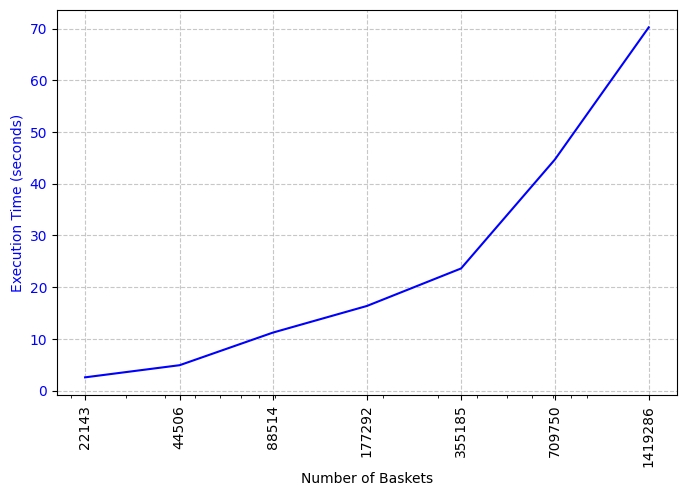
\includegraphics[width=0.7\textwidth]{n_baskets_vs_execution_time.png}
    \caption{Number of Baskets vs.\ Execution Time}
    \label{fig:n_baskets_vs_execution_time}
\end{figure}

\subsubsection{Effect of Minimum Support (min\_support) on Execution Time}

The second test examined execution time as the minimum support threshold decreased. The entire dataset was used, with \texttt{k\_max} held constant at 2. The tested \texttt{min\_support} values were 0.01, 0.005, 0.0025, 0.00125, 0.000625, 0.0003125, 0.00015625, and 0.000078125, each halving the previous threshold.  

Results presented in Figure \ref{fig:min_support_vs_execution_time} reveal different scalability patterns based on the number of frequent itemsets found:  
\begin{itemize}
    \item For small frequent itemset counts (up to 1,226 at \( \texttt{min\_support} = 0.00125 \)), execution time scales subline- arly.  
    \item For medium frequent itemset counts (up to 9,504 at \( \texttt{min\_support} = 0.00015625 \)), execution time scales~approximately linearly.  
    \item For large frequent itemset counts (above 25,000 at \( \texttt{min\_support} = 0.000078125 \)), execution time exhibits superlinear growth.  
\end{itemize}

Although execution time shows superlinear growth for the largest number of frequent itemsets found, the total runtime remains manageable at 459.17 seconds (approx.\ 7 minutes and 39 seconds). This further demonstrates the implementation's ability to efficiently process large-scale data, successfully handling around 200,000 baskets while identifying a substantial number of frequent itemsets, including singletons and pairs, within 8 minutes.

\begin{figure}[!ht]
    \centering
    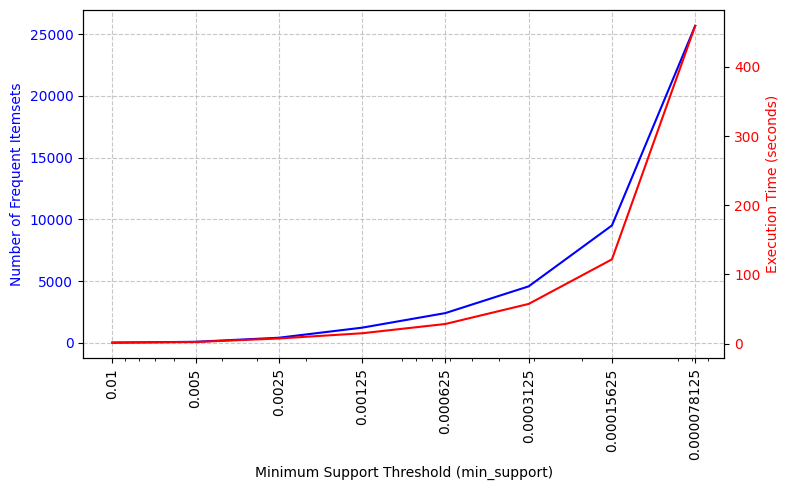
\includegraphics[width=0.7\textwidth]{min_support_vs_execution_time.png}
    \caption{Minimum Support Threshold vs.\ Execution Time}
    \label{fig:min_support_vs_execution_time}
\end{figure}

\subsubsection{Effect of Maximum Itemset Size (k\_max) on Execution Time}

The final test evaluated execution time for different values of \texttt{k\_max} while using the full dataset and a fixed min- imum support threshold of 0.1\%. The tested values of \texttt{k\_max} were 2, 3, 4, and 5.  

Results presented in Figure \ref{fig:k_max_vs_execution_time} indicate that execution time increases approximately linearly with the number of frequent itemsets found when \texttt{k\_max} increases from 2 to 3. Beyond this point, execution time grows slightly superlinearly, with the increase for \( \texttt{k\_max} = 5 \) being 1.5 times the increase in frequent itemsets found.

Despite this, finding frequent 4- and 5-itemsets remains computationally feasible, as even in the largest case, where nearly 9,000 frequent 5-itemsets are identified, execution time remains under 4 minutes.

\begin{figure}[!ht]
    \centering
    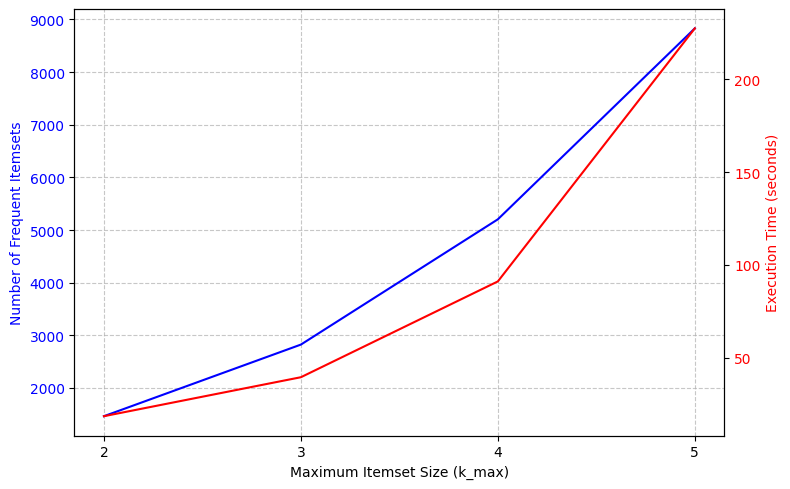
\includegraphics[width=0.7\textwidth]{k_max_vs_execution_time.png}
    \caption{Maximum Itemset Size vs.\ Execution Time}
    \label{fig:k_max_vs_execution_time}
\end{figure}

\section{Conclusions}\label{sec:5}

This project successfully implemented a parallelized version of the SON algorithm using Apache Spark, with~the Apriori algorithm employed for local itemset mining within partitions. The implementation was tested on a da- taset of Amazon book reviews to evaluate its effectiveness and scalability.

Mining for frequent pairs in a collection of 221,587 baskets with a support threshold of 0.01\% took approximately 4 minutes and identified 16,854 frequent itemsets. A subsequent association rule mining step allowed for the discovery of 10,500 rules with positive \textit{interest}, enabling the creation of a simple recommendation system.~In this system, for each book purchased by a user, another book could be suggested in the form of a banner:\ ``Other users often also liked ...''.

Further scalability tests demonstrated that execution time scales sublinearly with dataset size, indicating ef- ficient parallelization. When varying the minimum support threshold, execution time remained manageable even when identifying a large number of frequent itemsets, demonstrating the robustness of the approach. However, for extremely low support values, execution time increased superlinearly due to the exponential growth in fre- quent itemsets. Similarly, increasing \( k_{max} \) resulted in an approximately linear increase in execution time for small itemsets, while higher values led to a slightly superlinear increase. Despite this, the implementation re- mained computationally feasible, even for discovering frequent 4- and 5-itemsets.

Overall, the implementation scales well to large datasets and maintains efficiency across different parameter settings. Future improvements could focus on optimizing memory usage, dynamically adjusting partitioning strategies, and integrating more advanced pruning techniques to further improve execution time for low support thresholds and large itemset sizes. Additionally, applying the algorithm to different types of datasets could pro- vide further insights into its performance across various domains.

\printbibliography{references}
\end{document}